%%%%%%%%%%%%%%%%%%%%%%%%%%%%%%%%%%%%%%%%%%%%%%%%%%%%%%%%%%%%%%%%%%%%%%%%%%%%%%%
% Titel:   Realisation
% Autor:   Nicola K�ser
%%%%%%%%%%%%%%%%%%%%%%%%%%%%%%%%%%%%%%%%%%%%%%%%%%%%%%%%%%%%%%%%%%%%%%%%%%%%%%%
\chapter{Realisation}\label{ch:realisation}
%
	\section{Hardware}\label{s:hardware}
	Es wird je ein Ultraschallmodul vorne und eines hinten am Roboter montiert. Die Infrarotsensoren werden auch vorne und hinten, je nach Platz positioniert.
	Die Ultraschallmodule m�ssen nur an den \iic-Bus angeschlossen werden und ben�tigen keine weitere Hardware. F�r die Infrarotsensoren ist jedoch eine einfache Schaltung notwendig. Die zwei LEDs werden �ber ein Trimm-Potentiometer am Sensor angeschlossen, so kann gegebenenfalls die Schaltdistanz herabgesetzt werden.
	\image{content/image/todo}{scale=1}[Schema f�r Infrarotsensor][Schema f�r Infrarotsensor][pic:schema]
	Da die Schaltung nicht besonders aufwendig ist, sind die Printe als Veroboard-Aufbau realisiert. Auf Wunsch des Volumenkonzept-Teams wurden vorerst zwei Varianten des Printlayouts erstellt, eine quadratische- und eine l�ngliche Version. Da der Platz des kleinen Roboters relativ knapp ist, konnte so die bestm�gliche Option ausgew�hlt werden.
	\begin{figure}[H]
	\centering
	\begin{minipage}[t]{.49\textwidth}
		\centering
		
\includegraphics[scale=.2]{content/image/todo}
		\captionof{figure}[Hardwarevariante 1 - Quadratisch]{Variante 1 - Quadratisch}
		\label{pic:hardvarevariante1}
	\end{minipage}
	\begin{minipage}[t]{.49\textwidth}
		\centering
		
\includegraphics[scale=.2]{content/image/todo}
		\captionof{figure}[Hardwarevariante 2 - L�nglich]{Variante 2 - L�nglich}
		\label{pic:hardvarevariante2}
	\end{minipage}
	\end{figure}
	%
	Schlussendlich wurde zusammen die Entscheidung gef�llt vorne die l�ngliche- sowie zweimal die quadratische- und hinten einmal die quadratische Variante zu verwenden.
	%
	\section{Software}\label{s:software}
	F�r die Software wird das Echtzeitbetriebssystem FreeRTOS\footnote{Free real-time operating system} verwendet. Beim kleineren Roboter l�uft die Naherkennungs-Software auf dem RoboBoard zusammen mit weiteren Teilgebieten.
	%
		\subsection{Set\_SRF08\_address}\label{ss:set_srf08_address}
		Damit am gleichen \iic-Bus beide Ultraschallsensoren verwendet werden k�nnen, musste zuerst eine separate Software zum �ndern der Slave-Adresse erstellt werden. Der Ablauf der folgende:
		\begin{enumerate}
			\item �berpr�ffen ob neue Adresse g�ltig ist. Falls nicht, Programm nicht fortsetzten.
			\item Erste Pr�fsequenz zur Adress�nderung via \iic\ an Kommandoregister senden und definierte Zeit warten.
			\item Zweite Pr�fsequenz zur Adress�nderung via \iic\ an Kommandoregister senden und definierte Zeit warten.
			\item Dritte Pr�fsequenz zur Adress�nderung via \iic\ an Kommandoregister senden und definierte Zeit warten.
			\item Neue Adresse via \iic\ an Kommandoregister senden.
			\item Beim Aus- und erneuten Einstecken sollte nun die LED auf dem Modul mit dem zur neuen Adresse geh�renden Code (siehe Spezifikationen \cite{url:spec_srf08}) blinken.
		\end{enumerate}
		%
		Der vordere Sensor behielt seine Standard-Adresse (\hex{E0}), dem hinteren wurde die Adresse \hex{E2} neu zugewiesen.
		%
		\subsection{Rangefinder}\label{ss:rangefinder}
		F�r die Naherkennung wurden zwei Task implementiert, einer f�r die Infrarot- und einer f�r die Ultraschallsensoren.
		%
			\subsubsection{IR-Task}\label{sss:ir-task}
			Da ein Infrarotsensor lediglich einen GPIO\footnote{General purpose input/output} ben�tigt, ist der Taskablauf leicht zusammengefasst:
			\begin{enumerate}
				\item GPIOs initialisieren.
				\item Endlosschlaufe des folgenden Ablaufs:
				\begin{enumerate}
					\item Alle vier GPIOs lesen.
					\item �berpr�fen ob einer davon ein Hindernis erkennt.
					\begin{enumerate}
						\item Falls ein Hindernis erkannt ist, IR-Alarmflag setzen.
						\item Andernfalls IR-Alarmflag zur�cksetzen.
					\end{enumerate}
					\item Definierte Zeit warten, so dass der Task immer im gleichen Takt ausgef�hrt wird.
				\end{enumerate}
			\end{enumerate}
			%
			\subsubsection{US-Task}\label{sss:us-task}
			Der Task f�r die Ultraschallsensoren ist etwas komplizierter, wesshalb die Darstellung als Flussdiagram besser geeignet ist. F�r den \iic-Zugriff wurde das Mutex-Verfahren verwendet, zur �berschaubarkeit zeigen die Diagramme diesen Teil jedoch nicht.
			\image{content/image/flussdiagramm_us-task}{scale=1}[Flussdiagramm des US-Tasks][Flussdiagramm des US-Tasks][pic:flussdiagramm_us-task]
			\clearpage
			%
				\paragraph{Funktion setSRF08Range und setSRF08Gain}\label{par:setsrf08range_setsrf08gain}
				\ttodo{bla}
				\begin{figure}[H]
				\centering
				\begin{minipage}[t]{.49\textwidth}
					\centering
					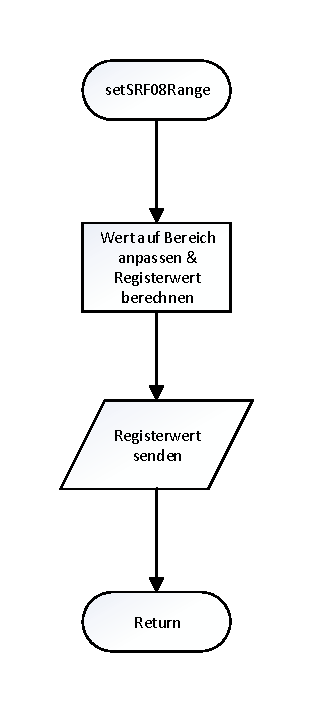
\includegraphics[scale=1]{content/image/flussdiagramm_setsrf08range}
					\captionof{figure}[Flussdiagramm der Funktion setSRF08Range]{Flussdiagramm der\newline Funktion setSRF08Range}
					\label{pic:flussdiagramm_setsrf08range}
				\end{minipage}
				\begin{minipage}[t]{.49\textwidth}
					\centering
					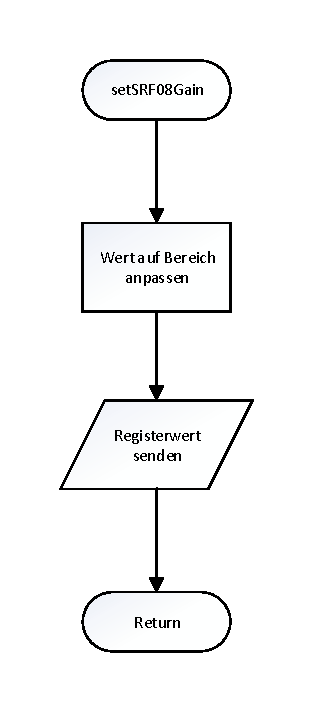
\includegraphics[scale=1]{content/image/flussdiagramm_setsrf08gain}
					\captionof{figure}[Flussdiagramm der Funktion setSRF08Gain]{Flussdiagramm der\newline Funktion setSRF08Gain}
					\label{pic:flussdiagramm_setsrf08gain}
				\end{minipage}
				\end{figure}
				%
				\paragraph{Funktion startSRF08Meas und readSRF08Meas}\label{par:startsrf08meas_readsrf08meas}
				\ttodo{bla}
				\image{content/image/flussdiagramm_startsrf08meas}{scale=1}[Flussdiagramm der Funktion startSRF08Meas][Flussdiagramm der Funktion startSRF08Meas][pic:flussdiagramm_startsrf08meas]
				%
				\image{content/image/flussdiagramm_readsrf08meas}{scale=1}[Flussdiagramm der Funktion readSRF08Meas][Flussdiagramm der Funktion readSRF08Meas][pic:flussdiagramm_readsrf08meas]
		%
